\subsection{Decompose Requirements}\label{subsec:decompose-requirements}

Decomposing requirements in HelixRM entails subdividing
broad business or marketing goals into specific, actionable
functional and system specifications.
This organised methodology guarantees that all elements of a
requirement are comprehensible, traceable, and manageable,
thereby optimising the development process.

\paragraph{Organize Requirements Hierarchically}
HelixRM allows users to establish and oversee hierarchical
arrangements for their requirements.
General requirements, such as “Improve user experience,” can
be further divided into more precise requirements, such as
“Ensure faster load times for pages” or “Enhance navigation intuitiveness.”
This hierarchy offers a clear visual depiction of how specific tasks
support broader objectives.

\paragraph{Create Traceability Links}
Traceability is a fundamental aspect of HelixRM, permitting
users to form direct connections between parent requirements
and their detailed sub-requirements.
For example, a business requirement can be linked to functional
specifications and related test cases.
This guarantees cohesion across all project components and
simplifies impact analysis for prospective changes.

\paragraph{Collaborate with Stakeholders}
HelixRM’s collaboration features promote smooth communication
throughout the decomposition process.
Team members and stakeholders can provide instantaneous feedback
and comments, ensuring transparency and agreement.
This engaging method minimizes ambiguity and fosters a
shared understanding of the requirements.

\paragraph{Use Templates and Reuse Requirements}
The platform improves efficiency by offering templates
and permitting the reuse of previously validated
requirements across various projects.
This not only saves time but also guarantees consistency
and adherence to organizational standards.

\paragraph{Analyze Risks and Dependencies}
As part of the decomposition process, HelixRM enables users to recognize and document potential risks and dependencies linked to particular requirements.
Integrated risk assessment tools support teams in proactively managing challenges that may arise during development.

\paragraph{Export for Wider Accessibility}
For external stakeholders or team members not directly utilizing HelixRM, decomposed requirements can be exported into widely used formats such as Word or Excel.
This feature guarantees that all pertinent parties can review, approve, or contribute to the refinement process.

By utilizing these functionalities, HelixRM ensures that intricate requirements are methodically disaggregated, fostering improved alignment, traceability, and implementation throughout the project lifecycle.


\begin{figure}[htbp]
    \centerline{
        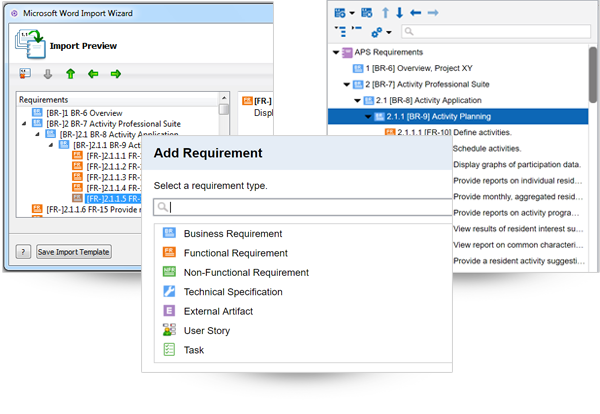
\includegraphics[width=\linewidth]
        {images/decompose}
    }
    \caption{HelixRM requirement decomposition.}
    \label{fig:fig}
\end{figure}